% Created by tikzDevice version 0.12.6 on 2024-09-18 12:11:01
% !TEX encoding = UTF-8 Unicode
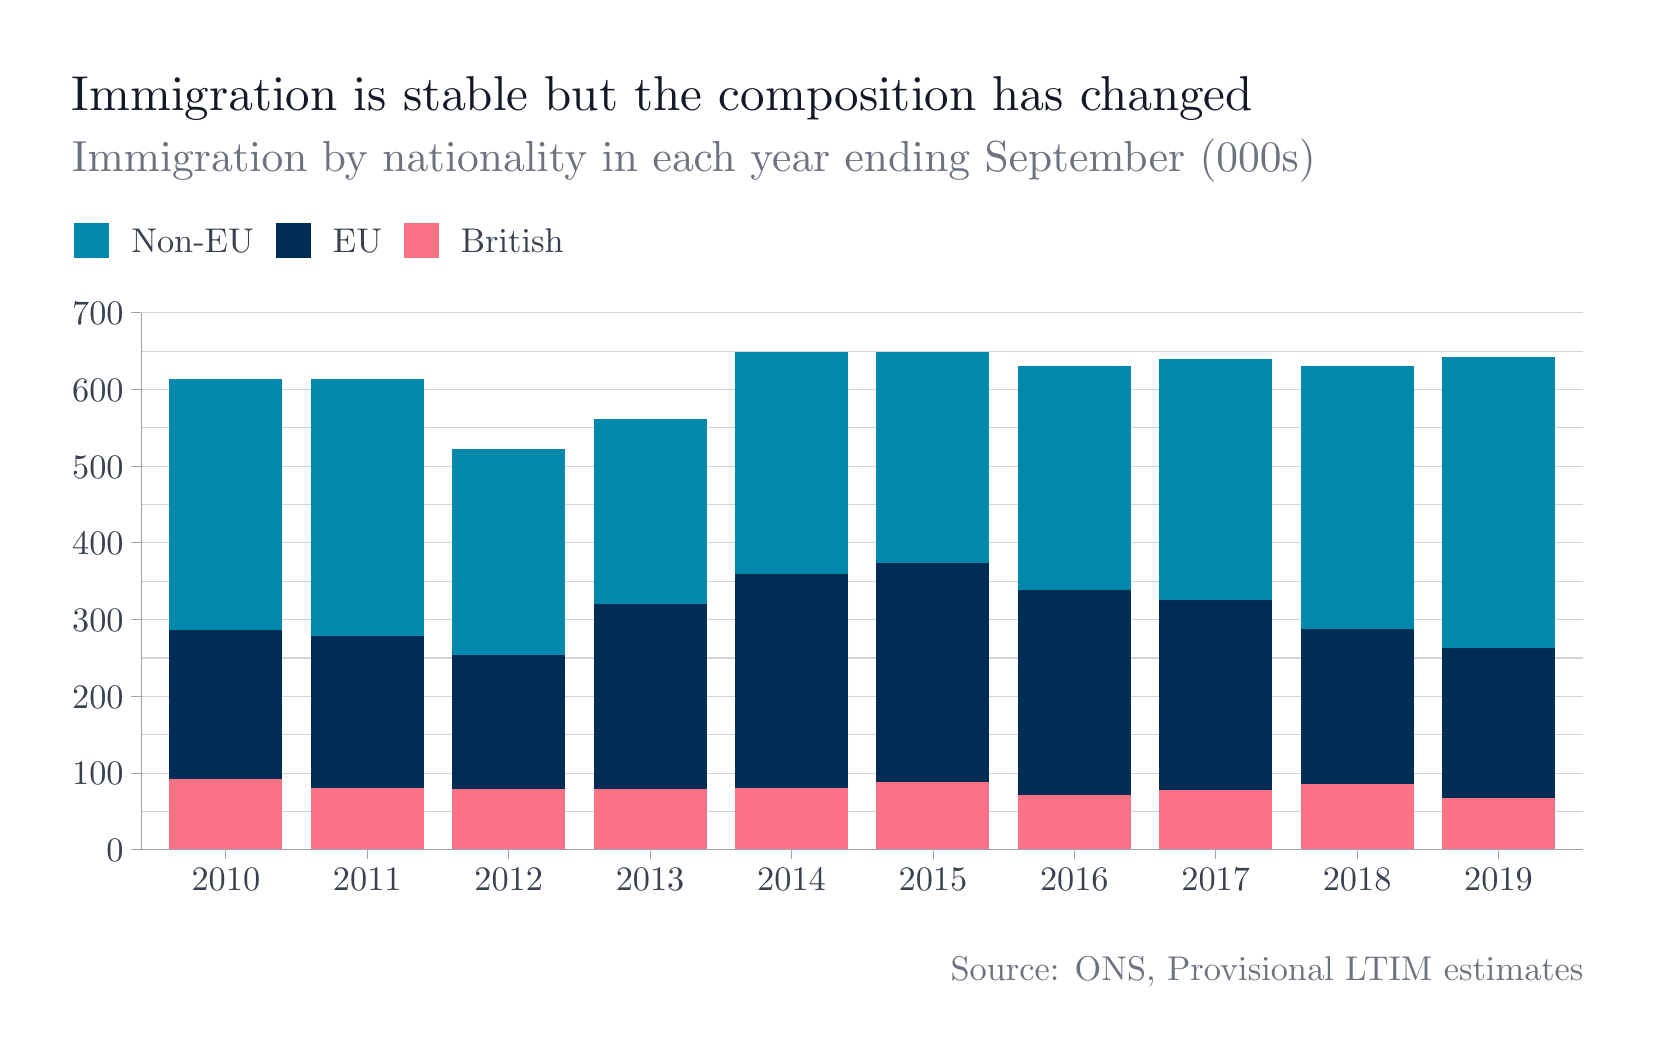
\begin{tikzpicture}[x=1pt,y=1pt]
\definecolor{fillColor}{RGB}{255,255,255}
\path[use as bounding box,fill=fillColor] (0,0) rectangle (578.16,361.35);
\begin{scope}
\path[clip] (  0.00,  0.00) rectangle (578.16,361.35);
\definecolor{drawColor}{RGB}{255,255,255}

\path[draw=drawColor,line width= 0.7pt,line join=round,line cap=round,fill=fillColor] (  0.00,  0.00) rectangle (578.16,361.35);
\end{scope}
\begin{scope}
\path[clip] ( 40.96, 64.27) rectangle (562.16,258.34);
\definecolor{drawColor}{RGB}{255,255,255}
\definecolor{fillColor}{RGB}{255,255,255}

\path[draw=drawColor,line width= 0.7pt,line join=round,line cap=round,fill=fillColor] ( 40.96, 64.27) rectangle (562.16,258.34);
\definecolor{drawColor}{RGB}{209,213,219}

\path[draw=drawColor,line width= 0.4pt,line join=round] ( 40.96, 78.13) --
	(562.16, 78.13);

\path[draw=drawColor,line width= 0.4pt,line join=round] ( 40.96,105.86) --
	(562.16,105.86);

\path[draw=drawColor,line width= 0.4pt,line join=round] ( 40.96,133.58) --
	(562.16,133.58);

\path[draw=drawColor,line width= 0.4pt,line join=round] ( 40.96,161.31) --
	(562.16,161.31);

\path[draw=drawColor,line width= 0.4pt,line join=round] ( 40.96,189.03) --
	(562.16,189.03);

\path[draw=drawColor,line width= 0.4pt,line join=round] ( 40.96,216.75) --
	(562.16,216.75);

\path[draw=drawColor,line width= 0.4pt,line join=round] ( 40.96,244.48) --
	(562.16,244.48);

\path[draw=drawColor,line width= 0.4pt,line join=round] ( 40.96, 64.27) --
	(562.16, 64.27);

\path[draw=drawColor,line width= 0.4pt,line join=round] ( 40.96, 92.00) --
	(562.16, 92.00);

\path[draw=drawColor,line width= 0.4pt,line join=round] ( 40.96,119.72) --
	(562.16,119.72);

\path[draw=drawColor,line width= 0.4pt,line join=round] ( 40.96,147.44) --
	(562.16,147.44);

\path[draw=drawColor,line width= 0.4pt,line join=round] ( 40.96,175.17) --
	(562.16,175.17);

\path[draw=drawColor,line width= 0.4pt,line join=round] ( 40.96,202.89) --
	(562.16,202.89);

\path[draw=drawColor,line width= 0.4pt,line join=round] ( 40.96,230.61) --
	(562.16,230.61);

\path[draw=drawColor,line width= 0.4pt,line join=round] ( 40.96,258.34) --
	(562.16,258.34);
\definecolor{fillColor}{RGB}{251,113,133}

\path[fill=fillColor] ( 51.18, 64.27) rectangle ( 92.05, 89.78);

\path[fill=fillColor] (102.27, 64.27) rectangle (143.15, 86.73);

\path[fill=fillColor] (153.37, 64.27) rectangle (194.25, 86.17);

\path[fill=fillColor] (204.47, 64.27) rectangle (245.35, 86.17);

\path[fill=fillColor] (255.57, 64.27) rectangle (296.45, 86.73);

\path[fill=fillColor] (306.67, 64.27) rectangle (347.55, 88.67);

\path[fill=fillColor] (357.77, 64.27) rectangle (398.64, 84.23);

\path[fill=fillColor] (408.86, 64.27) rectangle (449.74, 85.90);

\path[fill=fillColor] (459.96, 64.27) rectangle (500.84, 88.11);

\path[fill=fillColor] (511.06, 64.27) rectangle (551.94, 82.85);
\definecolor{fillColor}{RGB}{0,44,85}

\path[fill=fillColor] ( 51.18, 89.78) rectangle ( 92.05,143.84);

\path[fill=fillColor] (102.27, 86.73) rectangle (143.15,141.62);

\path[fill=fillColor] (153.37, 86.17) rectangle (194.25,134.69);

\path[fill=fillColor] (204.47, 86.17) rectangle (245.35,152.99);

\path[fill=fillColor] (255.57, 86.73) rectangle (296.45,164.08);

\path[fill=fillColor] (306.67, 88.67) rectangle (347.55,167.96);

\path[fill=fillColor] (357.77, 84.23) rectangle (398.64,158.26);

\path[fill=fillColor] (408.86, 85.90) rectangle (449.74,154.65);

\path[fill=fillColor] (459.96, 88.11) rectangle (500.84,144.12);

\path[fill=fillColor] (511.06, 82.85) rectangle (551.94,137.19);
\definecolor{fillColor}{RGB}{1,136,172}

\path[fill=fillColor] ( 51.18,143.84) rectangle ( 92.05,234.22);

\path[fill=fillColor] (102.27,141.62) rectangle (143.15,234.22);

\path[fill=fillColor] (153.37,134.69) rectangle (194.25,209.27);

\path[fill=fillColor] (204.47,152.99) rectangle (245.35,220.08);

\path[fill=fillColor] (255.57,164.08) rectangle (296.45,244.20);

\path[fill=fillColor] (306.67,167.96) rectangle (347.55,244.20);

\path[fill=fillColor] (357.77,158.26) rectangle (398.64,239.21);

\path[fill=fillColor] (408.86,154.65) rectangle (449.74,241.70);

\path[fill=fillColor] (459.96,144.12) rectangle (500.84,238.93);

\path[fill=fillColor] (511.06,137.19) rectangle (551.94,242.26);
\end{scope}
\begin{scope}
\path[clip] (  0.00,  0.00) rectangle (578.16,361.35);
\definecolor{drawColor}{RGB}{156,163,175}

\path[draw=drawColor,line width= 0.3pt,line join=round] ( 40.96, 64.27) --
	( 40.96,258.34);
\end{scope}
\begin{scope}
\path[clip] (  0.00,  0.00) rectangle (578.16,361.35);
\definecolor{drawColor}{RGB}{55,65,81}

\node[text=drawColor,anchor=base east,inner sep=0pt, outer sep=0pt, scale=  1.24] at ( 34.66, 59.99) {0};

\node[text=drawColor,anchor=base east,inner sep=0pt, outer sep=0pt, scale=  1.24] at ( 34.66, 87.71) {100};

\node[text=drawColor,anchor=base east,inner sep=0pt, outer sep=0pt, scale=  1.24] at ( 34.66,115.44) {200};

\node[text=drawColor,anchor=base east,inner sep=0pt, outer sep=0pt, scale=  1.24] at ( 34.66,143.16) {300};

\node[text=drawColor,anchor=base east,inner sep=0pt, outer sep=0pt, scale=  1.24] at ( 34.66,170.88) {400};

\node[text=drawColor,anchor=base east,inner sep=0pt, outer sep=0pt, scale=  1.24] at ( 34.66,198.61) {500};

\node[text=drawColor,anchor=base east,inner sep=0pt, outer sep=0pt, scale=  1.24] at ( 34.66,226.33) {600};

\node[text=drawColor,anchor=base east,inner sep=0pt, outer sep=0pt, scale=  1.24] at ( 34.66,254.05) {700};
\end{scope}
\begin{scope}
\path[clip] (  0.00,  0.00) rectangle (578.16,361.35);
\definecolor{drawColor}{RGB}{156,163,175}

\path[draw=drawColor,line width= 0.3pt,line join=round] ( 37.46, 64.27) --
	( 40.96, 64.27);

\path[draw=drawColor,line width= 0.3pt,line join=round] ( 37.46, 92.00) --
	( 40.96, 92.00);

\path[draw=drawColor,line width= 0.3pt,line join=round] ( 37.46,119.72) --
	( 40.96,119.72);

\path[draw=drawColor,line width= 0.3pt,line join=round] ( 37.46,147.44) --
	( 40.96,147.44);

\path[draw=drawColor,line width= 0.3pt,line join=round] ( 37.46,175.17) --
	( 40.96,175.17);

\path[draw=drawColor,line width= 0.3pt,line join=round] ( 37.46,202.89) --
	( 40.96,202.89);

\path[draw=drawColor,line width= 0.3pt,line join=round] ( 37.46,230.61) --
	( 40.96,230.61);

\path[draw=drawColor,line width= 0.3pt,line join=round] ( 37.46,258.34) --
	( 40.96,258.34);
\end{scope}
\begin{scope}
\path[clip] (  0.00,  0.00) rectangle (578.16,361.35);
\definecolor{drawColor}{RGB}{156,163,175}

\path[draw=drawColor,line width= 0.3pt,line join=round] ( 40.96, 64.27) --
	(562.16, 64.27);
\end{scope}
\begin{scope}
\path[clip] (  0.00,  0.00) rectangle (578.16,361.35);
\definecolor{drawColor}{RGB}{156,163,175}

\path[draw=drawColor,line width= 0.3pt,line join=round] ( 71.61, 60.77) --
	( 71.61, 64.27);

\path[draw=drawColor,line width= 0.3pt,line join=round] (122.71, 60.77) --
	(122.71, 64.27);

\path[draw=drawColor,line width= 0.3pt,line join=round] (173.81, 60.77) --
	(173.81, 64.27);

\path[draw=drawColor,line width= 0.3pt,line join=round] (224.91, 60.77) --
	(224.91, 64.27);

\path[draw=drawColor,line width= 0.3pt,line join=round] (276.01, 60.77) --
	(276.01, 64.27);

\path[draw=drawColor,line width= 0.3pt,line join=round] (327.11, 60.77) --
	(327.11, 64.27);

\path[draw=drawColor,line width= 0.3pt,line join=round] (378.21, 60.77) --
	(378.21, 64.27);

\path[draw=drawColor,line width= 0.3pt,line join=round] (429.30, 60.77) --
	(429.30, 64.27);

\path[draw=drawColor,line width= 0.3pt,line join=round] (480.40, 60.77) --
	(480.40, 64.27);

\path[draw=drawColor,line width= 0.3pt,line join=round] (531.50, 60.77) --
	(531.50, 64.27);
\end{scope}
\begin{scope}
\path[clip] (  0.00,  0.00) rectangle (578.16,361.35);
\definecolor{drawColor}{RGB}{55,65,81}

\node[text=drawColor,anchor=base,inner sep=0pt, outer sep=0pt, scale=  1.24] at ( 71.61, 49.40) {2010};

\node[text=drawColor,anchor=base,inner sep=0pt, outer sep=0pt, scale=  1.24] at (122.71, 49.40) {2011};

\node[text=drawColor,anchor=base,inner sep=0pt, outer sep=0pt, scale=  1.24] at (173.81, 49.40) {2012};

\node[text=drawColor,anchor=base,inner sep=0pt, outer sep=0pt, scale=  1.24] at (224.91, 49.40) {2013};

\node[text=drawColor,anchor=base,inner sep=0pt, outer sep=0pt, scale=  1.24] at (276.01, 49.40) {2014};

\node[text=drawColor,anchor=base,inner sep=0pt, outer sep=0pt, scale=  1.24] at (327.11, 49.40) {2015};

\node[text=drawColor,anchor=base,inner sep=0pt, outer sep=0pt, scale=  1.24] at (378.21, 49.40) {2016};

\node[text=drawColor,anchor=base,inner sep=0pt, outer sep=0pt, scale=  1.24] at (429.30, 49.40) {2017};

\node[text=drawColor,anchor=base,inner sep=0pt, outer sep=0pt, scale=  1.24] at (480.40, 49.40) {2018};

\node[text=drawColor,anchor=base,inner sep=0pt, outer sep=0pt, scale=  1.24] at (531.50, 49.40) {2019};
\end{scope}
\begin{scope}
\path[clip] (  0.00,  0.00) rectangle (578.16,361.35);
\definecolor{drawColor}{RGB}{255,255,255}
\definecolor{fillColor}{RGB}{255,255,255}

\path[draw=drawColor,line width= 0.7pt,line join=round,line cap=round,fill=fillColor] ( 16.00,272.34) rectangle (193.79,291.79);
\end{scope}
\begin{scope}
\path[clip] (  0.00,  0.00) rectangle (578.16,361.35);
\definecolor{drawColor}{RGB}{255,255,255}
\definecolor{fillColor}{RGB}{255,255,255}

\path[draw=drawColor,line width= 0.7pt,line join=round,line cap=round,fill=fillColor] ( 16.00,277.34) rectangle ( 30.45,291.79);
\end{scope}
\begin{scope}
\path[clip] (  0.00,  0.00) rectangle (578.16,361.35);
\definecolor{fillColor}{RGB}{1,136,172}

\path[fill=fillColor] ( 16.91,278.24) rectangle ( 29.55,290.89);
\end{scope}
\begin{scope}
\path[clip] (  0.00,  0.00) rectangle (578.16,361.35);
\definecolor{drawColor}{RGB}{255,255,255}
\definecolor{fillColor}{RGB}{255,255,255}

\path[draw=drawColor,line width= 0.7pt,line join=round,line cap=round,fill=fillColor] ( 88.85,277.34) rectangle (103.30,291.79);
\end{scope}
\begin{scope}
\path[clip] (  0.00,  0.00) rectangle (578.16,361.35);
\definecolor{fillColor}{RGB}{0,44,85}

\path[fill=fillColor] ( 89.75,278.24) rectangle (102.40,290.89);
\end{scope}
\begin{scope}
\path[clip] (  0.00,  0.00) rectangle (578.16,361.35);
\definecolor{drawColor}{RGB}{255,255,255}
\definecolor{fillColor}{RGB}{255,255,255}

\path[draw=drawColor,line width= 0.7pt,line join=round,line cap=round,fill=fillColor] (135.09,277.34) rectangle (149.55,291.79);
\end{scope}
\begin{scope}
\path[clip] (  0.00,  0.00) rectangle (578.16,361.35);
\definecolor{fillColor}{RGB}{251,113,133}

\path[fill=fillColor] (136.00,278.24) rectangle (148.64,290.89);
\end{scope}
\begin{scope}
\path[clip] (  0.00,  0.00) rectangle (578.16,361.35);
\definecolor{drawColor}{RGB}{55,65,81}

\node[text=drawColor,anchor=base west,inner sep=0pt, outer sep=0pt, scale=  1.24] at ( 37.45,280.28) {Non-EU};
\end{scope}
\begin{scope}
\path[clip] (  0.00,  0.00) rectangle (578.16,361.35);
\definecolor{drawColor}{RGB}{55,65,81}

\node[text=drawColor,anchor=base west,inner sep=0pt, outer sep=0pt, scale=  1.24] at (110.30,280.28) {EU};
\end{scope}
\begin{scope}
\path[clip] (  0.00,  0.00) rectangle (578.16,361.35);
\definecolor{drawColor}{RGB}{55,65,81}

\node[text=drawColor,anchor=base west,inner sep=0pt, outer sep=0pt, scale=  1.24] at (156.55,280.28) {British};
\end{scope}
\begin{scope}
\path[clip] (  0.00,  0.00) rectangle (578.16,361.35);
\definecolor{drawColor}{RGB}{107,114,128}

\node[text=drawColor,anchor=base west,inner sep=0pt, outer sep=0pt, scale=  1.57] at ( 16.00,309.32) {Immigration by nationality in each year ending September (000s)};
\end{scope}
\begin{scope}
\path[clip] (  0.00,  0.00) rectangle (578.16,361.35);
\definecolor{drawColor}{RGB}{17,24,39}

\node[text=drawColor,anchor=base west,inner sep=0pt, outer sep=0pt, scale=  1.77] at ( 16.00,331.42) {Immigration is stable but the composition has changed};
\end{scope}
\begin{scope}
\path[clip] (  0.00,  0.00) rectangle (578.16,361.35);
\definecolor{drawColor}{RGB}{107,114,128}

\node[text=drawColor,anchor=base east,inner sep=0pt, outer sep=0pt, scale=  1.24] at (562.16, 17.21) {Source: ONS, Provisional LTIM estimates};
\end{scope}
\end{tikzpicture}
